\chapter{Analysis of a low-background BEGe detector}
\label{chap:AnalysisBeGe}
	\section{Experimental setup}
	\label{sec:BeGeExperimentalSetup}

A custom 440~g PPC \textbf{B}road-\textbf{E}nergy \textbf{G}ermanium (BEGe) detector manufactured by Canberra Industries was deployed underground on 24~August~2009 in the Soudan Underground Laboratory in Soudan, MN.  The purpose of the deployment of this detector was to obtain low-threshold, low-background counting data to seek improved limits on WIMPs in the low-mass range ($\lesssim10$~GeV).  The design of this detector included several modifications to address backgrounds seen with a previous PPC used to obtain dark matter limits~\cite{Aalseth:2008aa}, including several internal mounting components replaced by ones constructed with cleaner materials by J.~Collar at the University of Chicago.  The detector was placed in the same shield as described in Section~\ref{sec:DeploymentPPC2SoudanIntro} with a few small changes.  The inner OFHC copper shield was replaced by old Pb bricks from the University of Chicago and a different PMT-based muon veto was placed around the external borated polyethylene shield.  %FixME contamination of bricks?

This chapter presents results from data taken with the BeGE detector underground from the time period beginning 4 December 2009 through 31 January 2010 for a total live-time of 54.375 days.  Results from a parallel analysis have been presented in~\cite{Aalseth:2010aa}.

	\section{Data acquisition and processing}
	\label{sec:BeGeDAQProcessing}
	
The DAQ system used was similar to the one used in~\cite{Aalseth:2008aa}.  The preamp of the BEGe included 2~signal outputs, an inhibit output generating a logic signal when the reset circuitry of the preamp was active, and a test input for waveform generator pulses.  The initial system was setup without the ability to digitize raw preamp traces, but a later upgrade on 1~Dec~2009 introduced additional hardware to take this data.  The readout system was a PCI-based National Instruments digitizer with 6~channels, sampling at 20~MS/s with a resolution of 8~bits.  This digitizer allowed selectable voltage ranges, enabling higher resolution at lower energies.  The acquisition software used was a Windows- and Labview-based program designed by J.~Collar.  

One of the preamp signal outputs was run into an analog spectroscopy amplifier with a 10$\mu$s shaping time.  Two outputs from this amplifier were input into the digitizer with different voltage ranges: -0.05$\to$0.05~V (high gain) and -0.25$\to$0.25~V (low gain).  The second preamp output was AC-coupled to a Phillips Scientific 777 fast (DC$\to$200~MHz) amplifier using a capacitor to yield a $\sim$50~$\mu$s decay time.  This stage provided a $\sim1\times$ gain and was used as a fan-out for two outputs to the next stage: (1) one output was input into a spectroscopy amplifier with 6~$\mu$s shaping time and then into the digitizer; (2) the other output was sent to another gain stage of the 777.  The two outputs from the fan-out of this stage were then input into two channels of the digitizer with different voltage ranges: -0.05$\to$0.05~V (high gain) and -0.25$\to$0.25~V (low gain).  The 777 allowed adjustment of the output offset, and so the baseline was set to be close to the upper maximum of the high-gain channel.  This was to maximize the dynamic range for digitizing the negative-going preamplifier pulses.  

The muon veto was composed of 10~flat panels situated around the outside of the polyethylene shield, with 6 on the sides and 4 covering the top.  The outputs of all the panels were coupled together and reduced to one channel, effectively OR-ing all the PMTs.  This single channel was then input into a discriminator with a threshold set to output logic pulses when any of the PMTs registered single photon.  This logic output was input into the last channel of the digitizer.  The outputs read into the DAQ system are detailed in Table~\ref{tab:SoudanDAQTable}.  All channels were digitized at 20~MHz with 8 bits, and each trace length was 8000 samples (400~$\mu$s) long.  The level-sensitive trigger was generated by the high-gain, 6~$\mu$s-shaped, channel~0.  When a pulse exceeded the trigger level in channel~0, all 6 channels were read out.  

\begin{table}
	\centering
	\begin{tabular}{|l|c|}
		\hline
		Channel & Characteristics \\
		\hline
		\hline
		0 & High-gain (0-3.5~keV), 6$\mu$s shaping \\
		\hline
		1 & High-gain (0-3.5~keV), 10$\mu$s shaping, triggering \\
		\hline
		2 & Low-gain (0-14~keV), 10$\mu$s shaping \\
		\hline
		3 & Muon-veto \\
		\hline
		4 & High-gain, AC-coupled preamp trace (unshaped) \\
		\hline
		5 & Low-gain, AC-coupled preamp trace (unshaped) \\
		\hline
	\end{tabular}
	\caption[DAQ Channel readout characteristics]
	{DAQ Channel readout characteristics. }
	\label{tab:SoudanDAQTable}
\end{table}

The inhibit output from the preamp was used as online veto by splitting the inhibit signal and using the `INHIBIT' inputs on the spectroscopy amplifiers.  When the logic is active on this INHIBIT input, the spectroscopy amplifier maintains the baseline of its output, effectively removing any trigger generated by a reset of the preamp.  It should be noted that, in contrast to the DAQ system described in Section~\ref{sec:DeploymentPPC2SoudanDAQSystem}, no timing information of the inhibit pulse was retained to perform a later estimate of deadtime.  Instead, during detector deployment it was found that the reset pulse rate was stable at $\lesssim$3~Hz, suggesting that differences in temperature did not affect this setup as profoundly as PPC2 (see Section~\ref{sec:DeploymentPPC2SoudanAnalysisCuts} or that the detector cold finger was more properly coupled to the liquid nitrogen.  %FixME Found out if JO still sees this at PNNL.

	The digitizer card maintained an internal buffer to store a set of events.  After 20~events were stored, data from the digitizer buffer were written to disk and files were cycled with name changes every 3 hours.  An automatic data management chain was setup similar to that described in Section~\ref{sec:DeploymentPPC2DataProcessing} with a run database used to facilitate the data processing.  Files were synchronized back to a server at the University of Washington where they were persisted on RAID-ed disks.  Once a file appeared on the UW server, a corresponding record was introduced into the database and this record was used to control and track further processing.  The processing progressed in a tiered fashion as follows:
		\begin{enumerate}
			\item[Tier 0:]  Raw data from the Labview DAQ system
			\item[Tier 1:]  ROOTified data - raw data converted to MGDO objects and stored in ROOT TFiles
			\item[Tier 2:]  Waveform processed data - extraction of waveform characteristics using MGDO Transforms
		\end{enumerate}
Details on the waveform processing are given in the following Sections: \ref{sec:BegeShapedProc}, \ref{sec:UnshapedWFProc}, and~\ref{sec:MuonProc}.  For more details regarding the MGDO objects and the framework of the analysis chain, see Appendix~\ref{app:MGDO}.
	
		\subsection{Shaped channel processing}
		\label{sec:BegeShapedProc}

The shaped channels (0, 1, and 2) were processed to extract amplitude information of the pulses.  These traces were first run through a 100~kHz low-bandpass filter to remove high-frequency noise and artifacts from the limited bit-depth of the digitizer.  Both extrema values, maximum and minimum, of each waveform were recorded and the baseline of each waveform was calculated using the first 280 $\mu$s (5600 samples).  The maximum was calculated both before and after the bandpass filter and both values saved; the minimum value was found on the unfiltered waveform.  The amplitude could then be calculated as the difference between the baseline and the maximum measured on the filtered waveform.  The minimum was saved to later analyze pulse health.

		\subsection{Unshaped channel processing}
		\label{sec:UnshapedWFProc}

The unshaped channels (4 and 5) were processed to extract information on the characteristics of the waveform, including baseline, extrema values, and rise-time information.  No bandpass frequency filter was used on the unshaped pulses to avoid removing the high-frequency components of the rising edge of the pulse.  The baseline was calculated using the first 5600 samples and the maximum and minimum were found for each pulse.  Calculating the rise-time of each pulse required de-noising using a time-invariant stationary wavelet transformation (SWT).  This process is described later in Section~\ref{sec:RisetimeCuts}.

		\subsection{Muon-veto channel}
		\label{sec:MuonProc}

The muon-veto channel digitized the logic output from a muon veto.  To process these waveforms, all the regions of each trace were found when the veto was logic positive.  Saving this information enabled any cut based upon the muon veto to be performed further down the analysis chain, retaining flexibility in determining parameters for such a cut.  However, due to the high count rate of the muon veto and therefore the reduction in live-time any cut from this veto would create, it was decided to not use any cuts based upon results from this channel in the analysis.


	\section{Data analysis}
	\label{sec:BeGeDataAnalysis}
		\subsection{Triggering efficiency}
		\label{sec:BeGeTrigEff}

FixME - Flesh out trigger efficiency

The trigger efficiency of the DAQ system was measured by scanning a pulser of known amplitude through the threshold.  The data was then fit to the function:
			\[
			1 - \frac{\operatorname{erf} \left(s(V-\sigma)\right)}{2}
			\]
where $V$ is in volts.  This yielded the results: $\sigma = 7.137\times10^{-3}\pm8\times10^{-6}$ and $s = -1.772\times10^{3}\pm28$.  Results are shown in Figure~\ref{fig:BeGeTriggeringEfficiency}.

			\begin{figure}
				\centering
				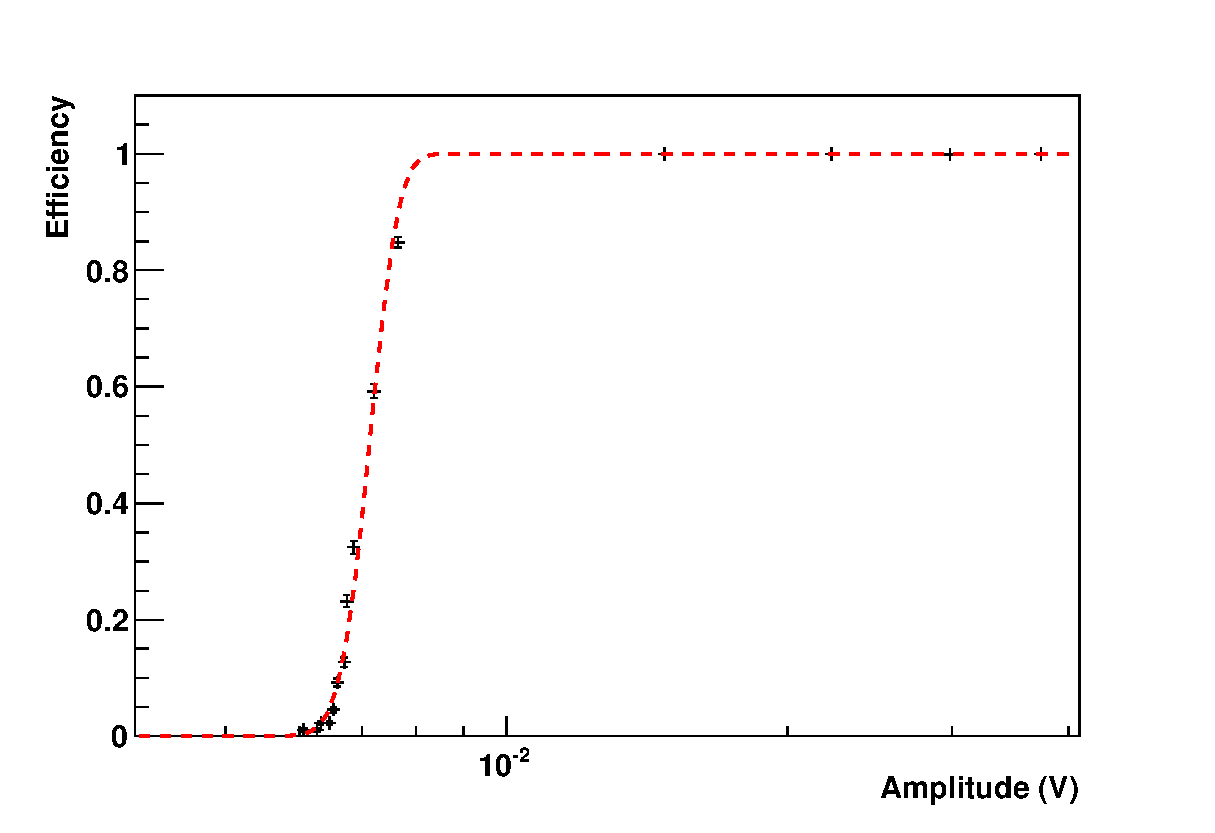
\includegraphics[width=0.9\textwidth]{energy_efficiency_bege}
				\caption[BeGe triggering efficiency measured with a pulser]
				{BeGe triggering efficiency measured with a pulser.  Error bars are binomial.}
				\label{fig:BeGeTriggeringEfficiency}
			\end{figure}

		\subsection{Resolution of results}

FixME - Flesh out measurement of widths of gaussians

The inherent noise was measured using a pulser as well as x-ray lines.  The results of these measurements were folded into the following equation:

			\begin{equation}
				\sigma = \sqrt{\sigma_{elec}^{2} + E \eta F}
				\label{eqn:SigmaEqn}
			\end{equation}

to measure the intrinsic electronic noise $\sigma_{elec}$ and estimate the Fano factor $F$.  $E$ is the energy in keV, $\eta$ the amount of energy required to generate an electron-hole pair (2.96 eV).  $\sigma_{elec}$ was found to be $70.48\pm0.54$~eV and $F$ was estimated as $0.166\pm0.014$.  Results are shown in Figure~\ref{fig:BeGeResPlot}.

			\begin{figure}
				\centering
				%\includegraphics[width=0.8\textwidth]{Figures/resolution_plot1}
				\caption[BeGe resolution versus energy]
				{BeGe resolution versus energy.  Red is measured and fit intrinsic electronic noise, 
				black points are measured resolution from x-ray lines, black line is a fit to 
				Eqn.~\ref{eqn:SigmaEqn}.}
				\label{fig:BeGeResPlot}
			\end{figure}

		\subsection{Energy calibration}

The energy calibration was determined by fitting the high-energy channel simultaneously to the peaks listed in Table~\ref{tab:XRayLines} yielding a linear equation:

			\[
			E_{ion} (keV) = a V + b
			\]  

with $a = 63.81\pm0.25$~(keV/V) and $b = -0.014551\pm0.016$~keV.


	
	
	\section{Microphonics and Noise Cuts}
     	\label{sec:MicroCuts}	

FixME - Explain microphonics cuts, fleshing out the details of exactly what is done here, and how the efficiencies are estimated.  

	Vibrations in detector components, such as the cryostat, cold-finger, or crystal mount, can induce electronic signals due to the changing capacitance created by the movement of components.  These electronic deviations can generate extra noise at low energies (threshold to a few keV) possibly obscuring signal in that region.  Morales et al.~developed a technique to mitigate this class of events, taking advantage of the fact that microphonics tend to have characteristics (e.g.~rise-time, fall-time, baseline shift) significantly different from events arising from charge collection in the crystal~\cite{Morales1992410}.  This procedure analyzes the ratio of amplitudes from two signal channels with different shaping times  and accepts or rejects events based upon their deviation from the expected ratio.  This expectation can be determined by using a source or a pulser at low amplitudes.  
	
	In this application, the ratio of two 

			\begin{figure}
				\centering
				%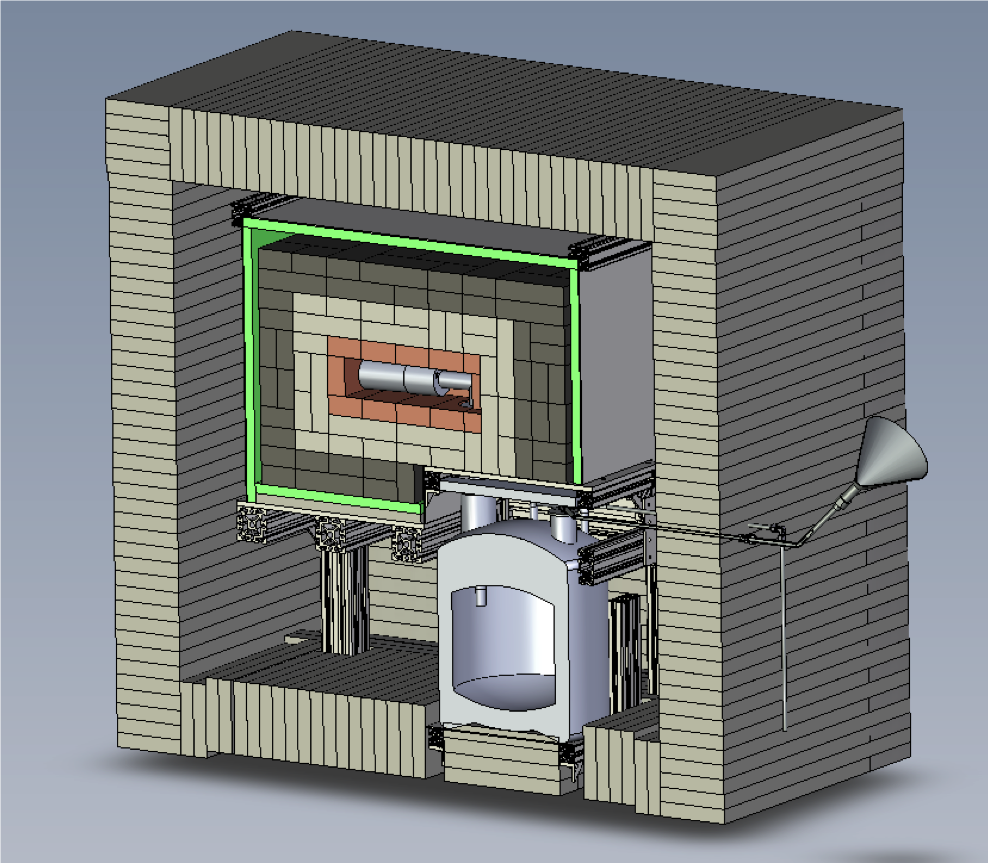
\includegraphics[width=0.9\textwidth]{PPC2DesignSchematicAll}
				\caption[BeGe microphonics cuts]
				{Microphonics cuts using the ratio of outputs from two different spectroscopy amplifiers.}
				\label{fig:RatioOfShapedChannels}
			\end{figure}


	\section{Risetime cuts}
     	\label{sec:RisetimeCuts}	

		\subsection{Wavelet denoising}
	     	\label{sec:RisetimeCutsWaveletDenoise}
					
	As the amplitude-to-noise ratio of waveforms shrinks at low energies, calculating the rise-time becomes more sensitive to the magnitude of the noise.   Denoising via a simple bandpass filter is undesirable when both signal and noise are distributed across similar frequency bands as the signal-to-noise ratio will not be enhanced by removing particular frequencies.  When calculating the rise-time of a pulse, a bandpass filter can greatly attenuate the high frequencies present in the rising edge of the pulse.  Wavelet shrinkage provides methodology to reduce noise on a generic function (see e.g.~\cite{Don95aa,Don95bb}) when the function and and noise occupy the same frequency space.  The algorithm follows:
				\begin{enumerate}
					\item Choose a wavelet basis.
					\item Perform a wavelet transformation using the chosen basis to a level $n$, 
					obtaining $n$ sets of detail and approximation coefficients.
					\item Apply thresholding to the detail coefficients.
					\item Perform an inverse transformation.
				\end{enumerate}
	In this particular application it is necessary to use a translation-invariant version of the wavelet transformation called a Stationary Wavelet Transformation (SWT) (see~\cite{Coif95aa,Naso95aa}).  The SWT performs transformations at all possible translations for a given data set and basis wavelet.  A subsequent inverse SWT effectively averages these together, avoiding artifacts induced by any chosen origin.  
	
	For this wavelet analysis, the python package PyWavelets~\cite{PyWave} was used.  Since an implementation of the inverse SWT was missing from this distribution, the necessary extension to the package was written (see Section~\ref{sec:WaveformProcMGDO}.  A Haar wavelet was chosen as a basis wavelet due to its simplicity and asymmetry.  Thresholds for each set of detail coefficients were calculated using a pure-noise waveform training set of length $j$.  For each noise waveform $x^{(i)}$, a 6-level SWT was used to generate $D_{n}^{(i)}$ and the thresholds were calculated for each level $n$ according to the equation proposed by Donoho and Johnston~\cite{Don95ad}:
	
				\begin{equation}			
					\tau_{n}^{(i)} = \sigma_{n}^{(i)} \sqrt{2 \log N^{(i)}}
				\end{equation}			
				\[
					\sigma_{n}^{(i)} = \frac{\operatorname{MAD}\left(D_{n}^{(i)}\right)}{0.6745}
				\]
with $N^{(i)}$ the length of waveform, $x^{(i)}$, and MAD is the median average deviation.  The threshold at a level $n$ was then defined as $\tau_{n} = 0.8 \max(\tau_{n}^{(0)},...,\tau_{n}^{(j)})$.  An example of the coefficients calculated using a 6-level SWT is shown in Figure~\ref{fig:RisetimeCutsWaveletDecompositionOfPulse}.  This figure also includes the thresholds calculated at each level, denoted by dashed lines.  

Noise reduction was implemented by applying hard thresholding to each set of detail coefficients.  In this technique, all coefficients $D_{n}$ with an absolute value less than the threshold $\tau_{n}$ were set to zero.  Coefficients above this threshold value were unchanged.  The resultant coefficients were then used in an inverse SWT to produce a de-noised waveform.  An example of the wavelet de-noising is shown in the top figure of Figure~\ref{fig:RisetimeCutsExampleOfPulse}.
	
			
				\begin{figure}
					\centering
					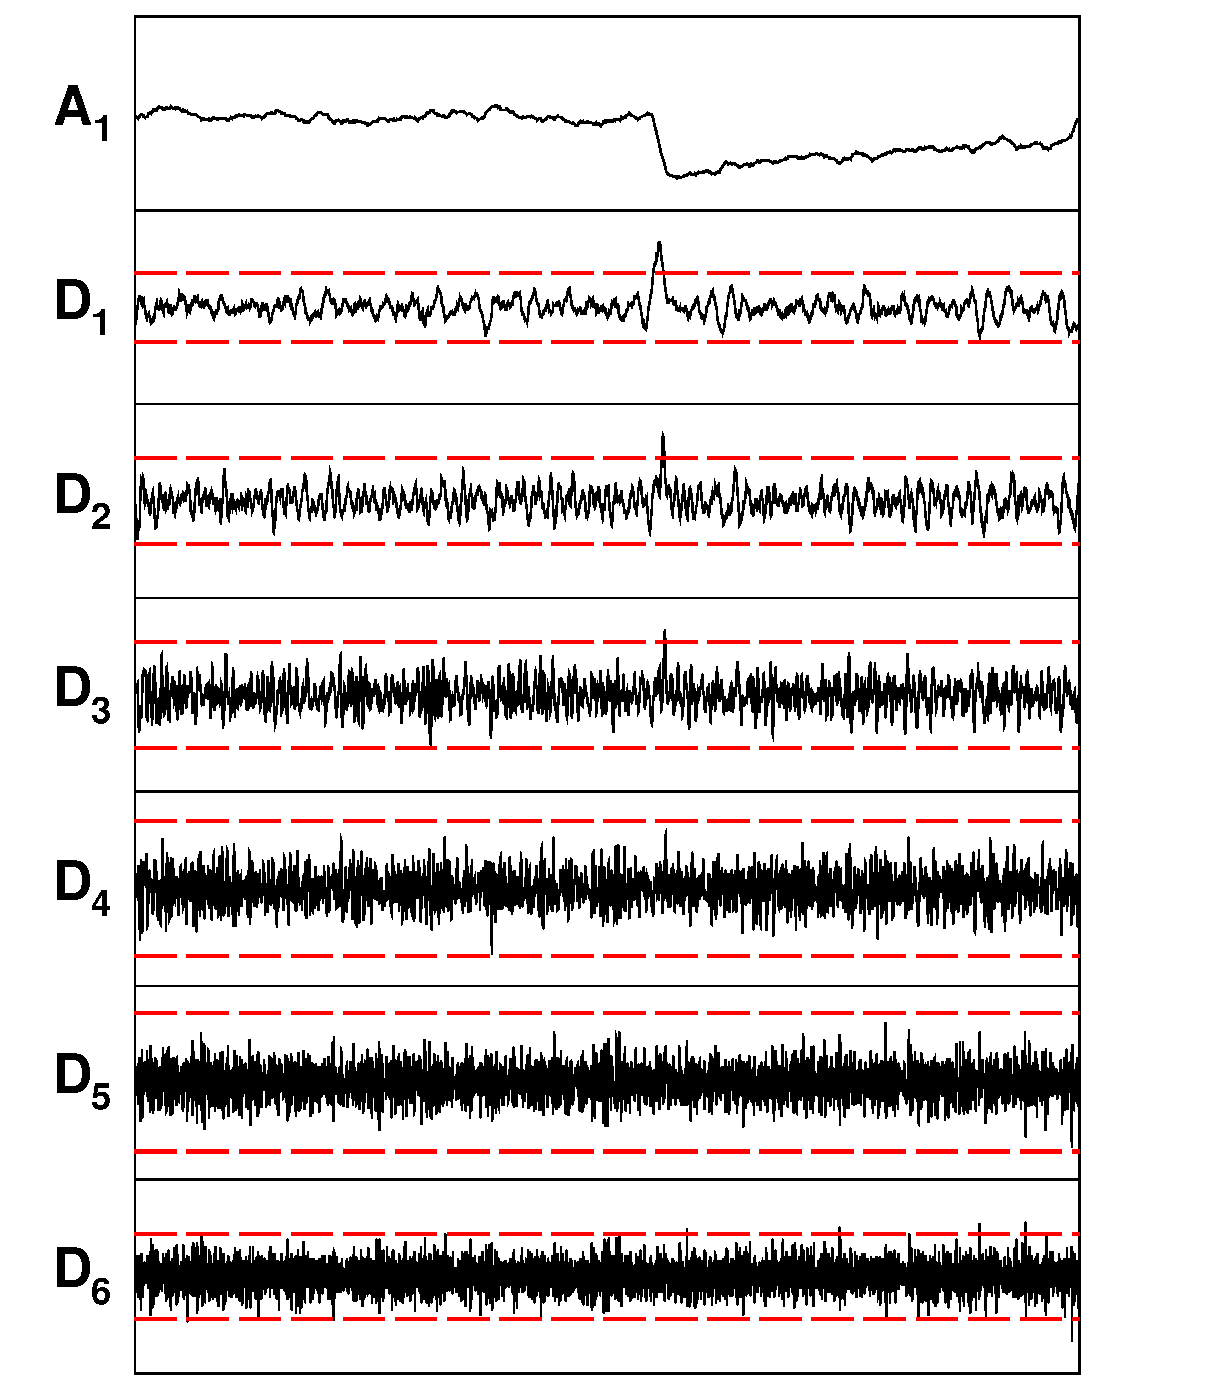
\includegraphics[width=0.95\textwidth]{ExampleWavelet}
					\caption[Example wavelet decomposition of pulse]
					{Example wavelet decomposition of pulse in Figure~\ref{fig:RisetimeCutsExampleOfPulse}.  
					A$_{1}$ denotes the first-level
					 approximation coefficients, the D$_{n}$ denote the detail coefficients at the $n$th level of the 6-level stationary wavelet 
					 transformation.  Dashed lines indicate the thresholding used for each set of detail coefficients.}
					\label{fig:RisetimeCutsWaveletDecompositionOfPulse}
				\end{figure}					

		\subsection{Risetime calculation}
		\label{sec:RisetimeCalculation}
	The denoising process ensured that the waveforms be ready for rise-time calculations.  After de-noising, the smoothed derivative of the waveform was generated using a Savitzky-Golay derivative filter~\cite{Sav64aa}.  The extremum of the derivative - in this case the minimum since the pulse was negative-going - was then found and used to determine the middle of the rising edge, $p_{m}$.  The full-width at half maximum (FWHM) was calculated and used to estimate the beginning and end of the rise of the waveform: the beginning, $p_{b} = p_{m} - 1.5\times$FWHM and the end, $p_{e} = p_{m} + 1.5\times$FWHM.  The baseline and amplitude of the pulse were each found by averaging over 1~$\mu$s (20~samples) beginning at $p_{b} - (1~\mu$s) and $p_{e}$, respectively.  These values were used to estimate the amount of time it took the pulse to rise 10\%$\to$90\% in amplitude.  Linear interpolation was used to refine the time values which came between digitization points.  An example of this calculation, using the same pulse as in Figure~\ref{fig:RisetimeCutsWaveletDecompositionOfPulse}, is shown in Figure~\ref{fig:RisetimeCutsExampleOfPulse}.  
		
				\begin{figure}
					\centering
					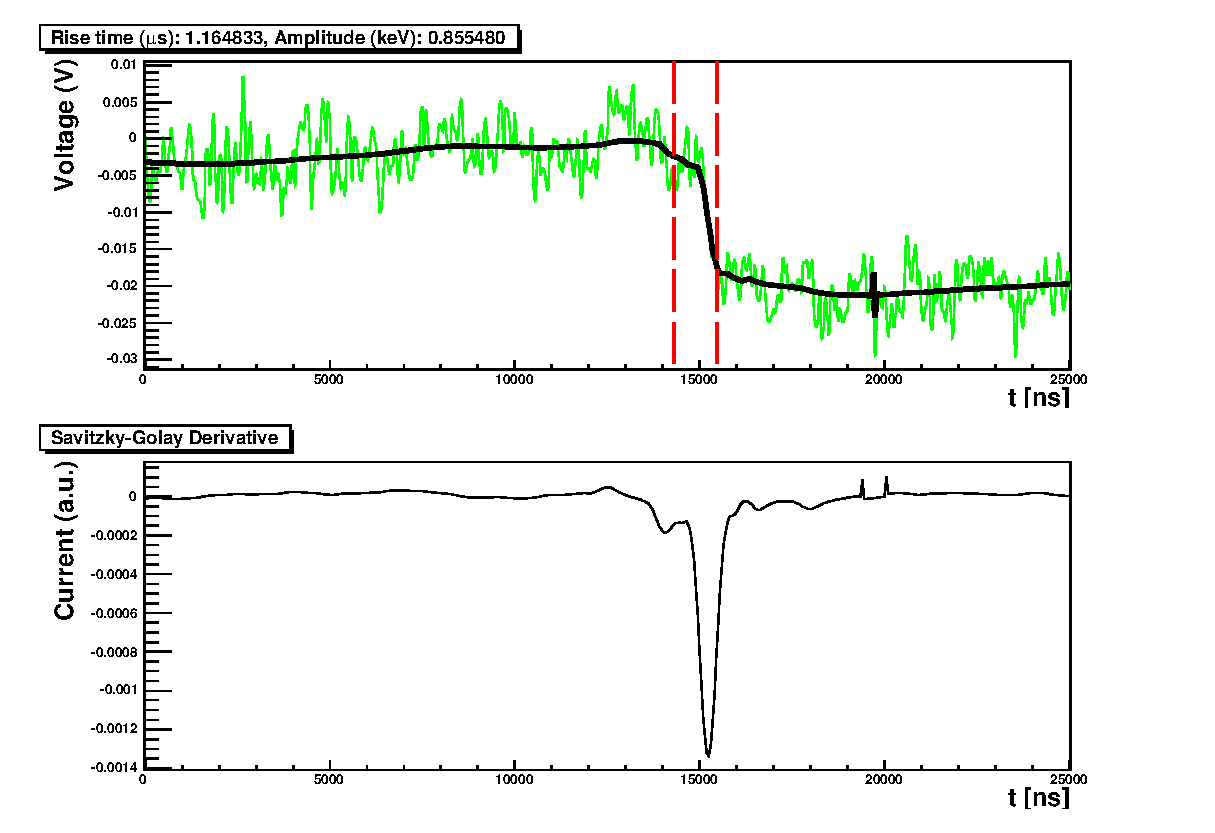
\includegraphics[width=0.9\textwidth]{ExampleWaveform0}
					\caption[Example of rise-time calculation technique applied to a preamp trace]
					{Example of rise-time calculation technique applied to a preamp trace.  
					The top shows the raw and denoised waveforms, and the vertical dashed lines represent the result 
					of the rise-time calculation.  The bottom plot shows the smoothed derivative of the trace calculated 
					using a Savitzky-Golay filter~\cite{Sav64aa} of degree~2, width~6.}
					\label{fig:RisetimeCutsExampleOfPulse}
				\end{figure}					

			\subsection{Risetime simulation}
			\label{sec:RisetimeSimulation}
	
	To investigate how a cut based upon rise-time affected the spectrum, it was necessary to perform a simulation of the rise-time calculation on waveforms similar to the data.  The idea was to produce waveforms with similar characteristics (i.e. rise-time, noise) as seen in the detector and run them through the same algorithm used to analyze the detector data.  The waveform was generated by taking a tail pulse of 0~rise-time and running it through a digital low-pass RC filter.  The RC constant in the filter was tuned to reproduce the rise-time of ``fast'' pulses seen in the data.  In general this would not precisely reproduce all the characteristics of the detected pulses, but since the only parameter of interest was the rise-time it was reasonable to choose such a simple pulse construction.  Later systematic tests (Section~\ref{sec:RisetimeSystematicTests}) verified that it was sufficient.  
	
	The electronic noise of the detector was measured by looking at the baseline of all pulses and taking the average of power spectra for each preamp trace channel.  Once the average power spectrum was determined, it was possible to use this to add noise to the simulated pulse through the techniques outlined in~\cite{WanThesis08} by Wan Tseung.  Essentially, a measurement of an average power spectrum, $\Omega = X^{2} + Y^{2}$ where $X$ and $Y$ are the real and imaginary components of the Fourier Transform, gives you an average value $\mu_{i}$ at a frequency bin $i$.  If there is no phase information in the noise (i.e.~$\tan^{-1} (X_{i}/Y_{i})$ is flatly distributed), $X_{i}$ and $Y_{i}$ are gaussian-distributed variables around 0 with the same standard deviation, $\sigma_{i}$, which is related to the average value of bin $i$ via  $\mu_{i} = 2 \sigma_{i}^{2}$.  Therefore, for each simulated pulse, a noise waveform was generated in frequency space, transformed to the time domain using a discrete inverse Fourier Transform, and added to the original simulated pulse.  
	
	Since the energy of each event was determined using the amplitude of shaped pulses, it was necessary to determine a relationship between amplitudes of the shaped and unshaped low-gain channels (channel 1 and channel 4) and the amplitudes of the shaped and unshaped high-gain channels (channel 2 and channel 5).  This was done by fitting the relationship from data, an example of which is shown in Figure~\ref{fig:Risetimechan2vschan4}.  Additionally, the waveforms' position in the trace window exhibited a dependence on the energy of the event: for events of smaller amplitude the trigger tended to arrive later so that the waveform moved left in the trace window.  This dependence was measured by tracking the start of the pulse in the trace window versus amplitude and fitting it to an empirical polynomial (see Figure~\ref{fig:TriggerPositionDependence}).  This information was folded back into the simulation to control the starting point of the pulse given its amplitude.
	
					\begin{figure}
						\centering
						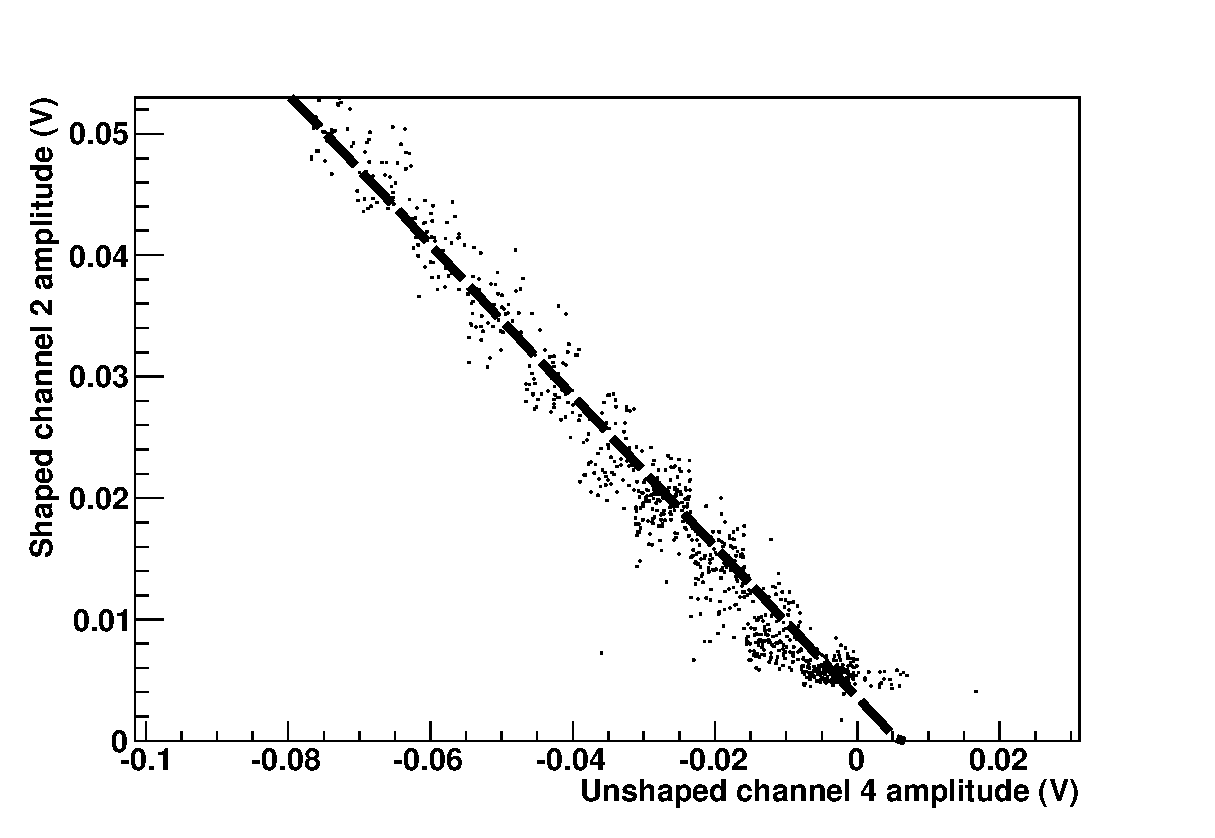
\includegraphics[width=0.9\textwidth]{chan4amplitude_vs_chan1}
						\caption[Comparison between the amplitudes in the unshaped and shaped BeGe channels]
						{Comparison between the amplitudes in the unshaped channel 4 and shaped channel 1.  
						The line is a linear fit to the data.}
						\label{fig:Risetimechan2vschan4}.
					\end{figure}
					
					\begin{figure}
						\centering
						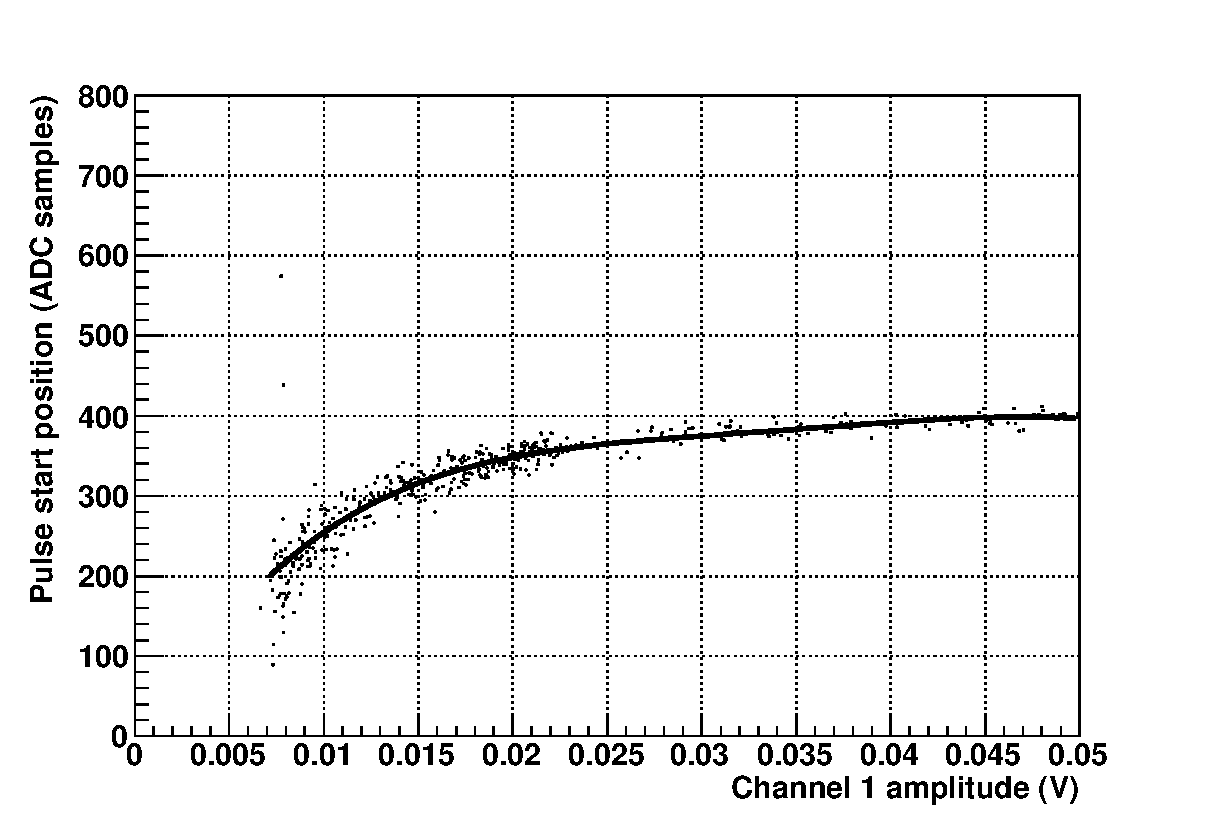
\includegraphics[width=0.9\textwidth]{start_pulse_vs_energy}
						\caption[Comparison between the start of the preamp pulse rise-time and the amplitude of the shaped channel for the BeGe]
						{Comparison between the start of the preamp pulse rise-time and the amplitude of the shaped
						 channel.  The line is a fourth-order polynomial fit which is used to parameterize this relationship.}
						\label{fig:TriggerPositionDependence}.
					\end{figure}					
	
	Once the simulated pulses were generated, they were run through the same analysis chain as the waveforms from the detector, in particular through the rise-time calculation algorithms described earlier in this section.  The amplitude of the pulses was sampled according to the triggering efficiency measured in Section~\ref{sec:BeGeTrigEff}.  Two simulations were run, one for each the high- and low-gain set of channels, for $\sim$5M events.  These results were then used to calculate contours of particular acceptances, 40, 50, 60, 70, 80, 90, 95, and 99\%.  Results of the simulation for the low-gain channel are shown in Figure~\ref{fig:RisetimeSimulation} along with a calculated 99\% acceptance contour.  The acceptance region defined as all waveforms having a calculated rise-time less than or equal to the calculated contour.  
					
				\begin{figure}
					\centering
					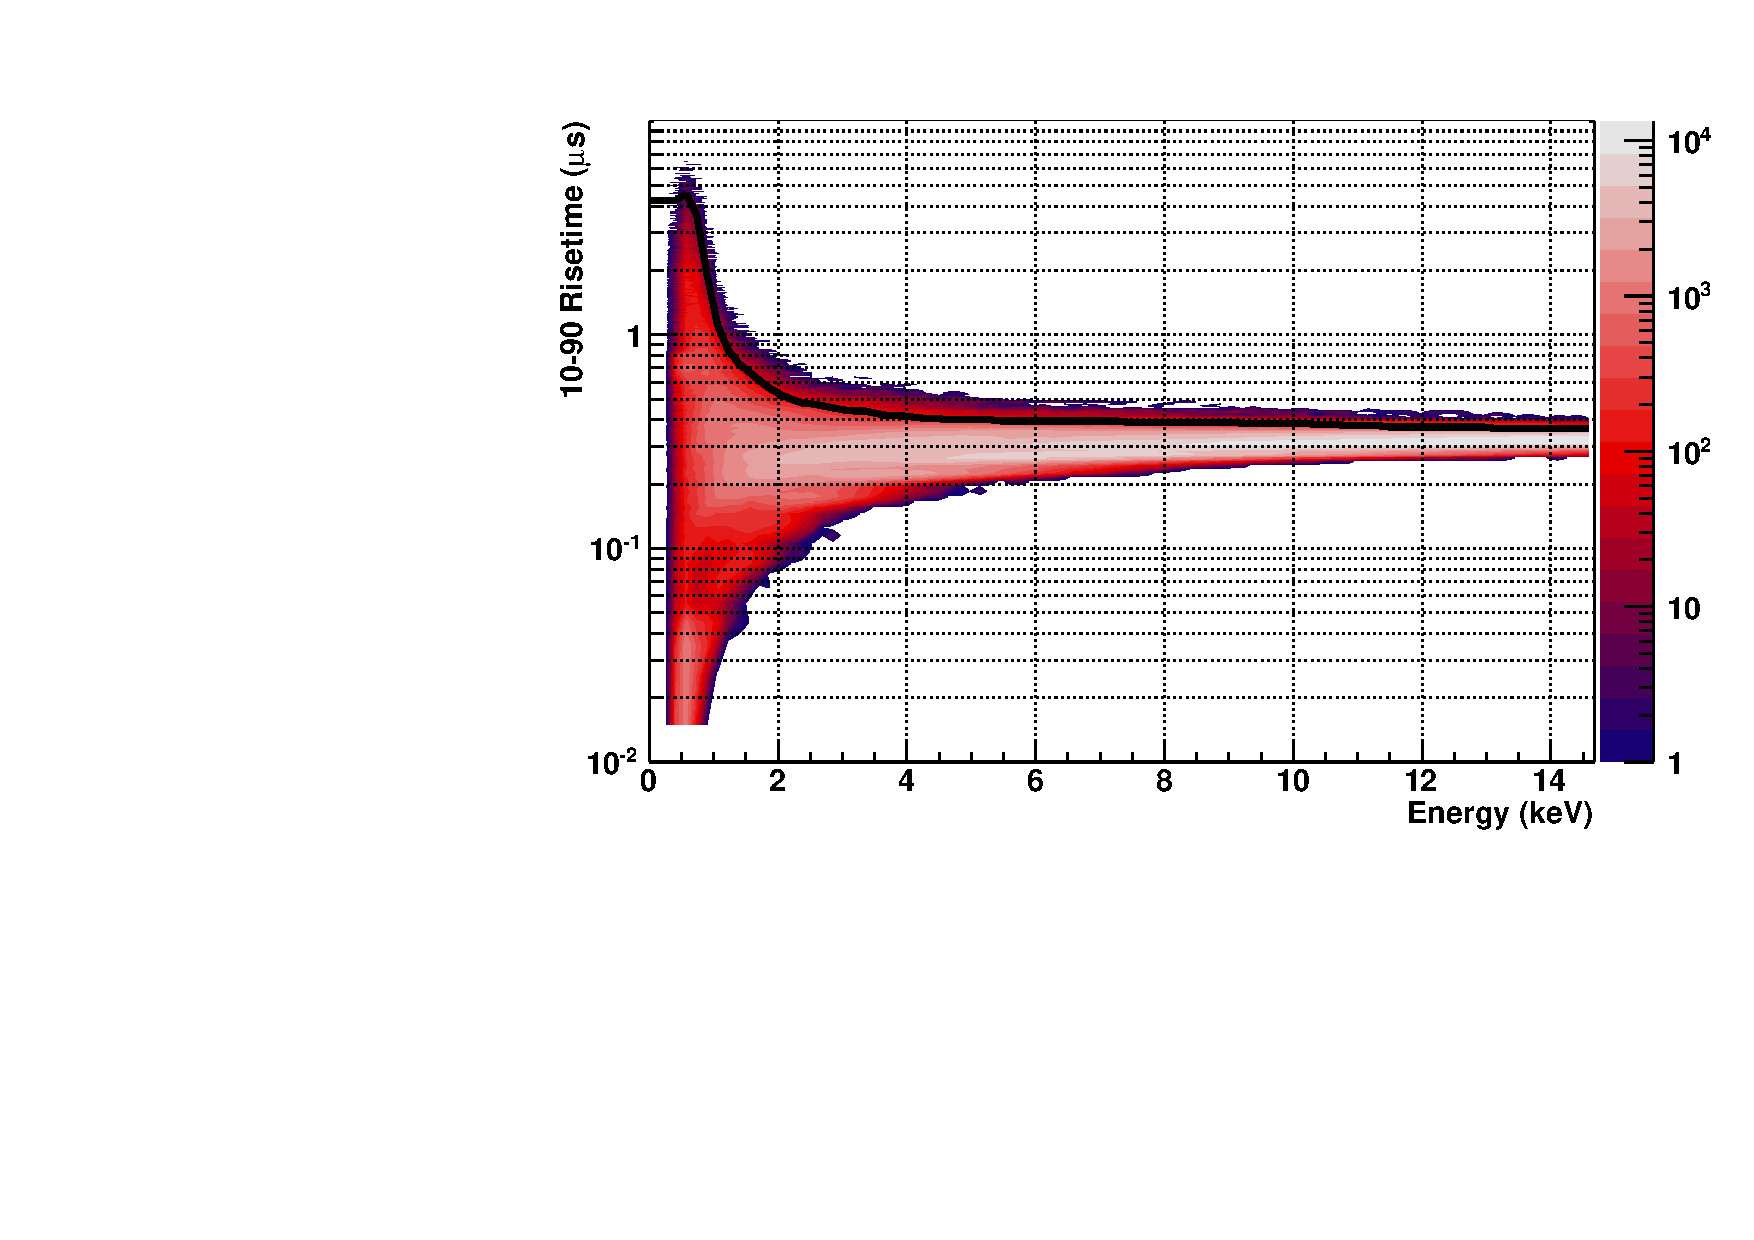
\includegraphics[width=0.9\textwidth]{risetime_cut_chan5_nice}
					\caption[Simulation of calculated rise-time for the low-gain channel of the BeGe]
					{Simulation of calculated rise-time for the low-gain channel of the BeGe.}
					\label{fig:RisetimeSimulation}
				\end{figure}	
	
		\subsection{Risetime systematic tests}
		\label{sec:RisetimeSystematicTests}	
	
	Systematic tests of the cuts were performed to verify the simulation performed adequately and that the cuts behaved as expected.  To do this, cuts of different acceptance were applied to the data set, and an unbinned maximum likelihood fit of the cut data set was performed to measure how the cut affected the different features in the data.  This fit included all x-ray lines (see Table~\ref{tab:XRayLines}) and a background with a flat component and an exponential component.  The fit equation was then:

					\begin{equation}
						b_{1} \exp\left(c_{1} E\right) + b_{2} + \sum^{xrays}_{i} \frac{a_{i}}{\sigma_{i}\sqrt{2 \pi}} 
							\exp\left(-\frac{(E - \mu_{i})^{2}}{2 \sigma_{i}^{2}}\right)
						\label{eqn:InitialFitEqn}
					\end{equation}

where $b_{1}$ and $b_{2}$ are the exponential and flat background amplitudes respectively, $c_{1}$ is the exponential constant and the sum is over the xray lines present in the fit.  The amplitudes of all components ($a_{i}$, $b_{1}$, $b_{2}$) and the exponential constant were allowed to float independently.  The parameters ($\mu_{i}$ and $\sigma_{i}$) of the x-ray lines were allowed to float in a small range around their expected values.  

These fits were performed for data sets with the entire set of cuts, including:

					\begin{enumerate}
						\item only LN fills
						\item LN fills and microphonics cuts
						\item LN fills, microphonics cuts, and risetime cuts varying between 40\% and 99\%.
					\end{enumerate}

These fits were performed for both high-energy and low-energy channels, an example of a fit for each channel is given in Figure~\ref{fig:BeGeFitExample}.  A calculation of the relative percentage remaining for each component was made using the cut LN-fills-plus-microphonics as a reference.  This calculation gives a metric for determining the validity of each cut; for example, a rise-time cut with a calculated 70\% acceptance efficiency should retain 70\% of the counts in the x-ray lines and remove an unknown but larger percentage of the counts in the background components (flat plus exponential).  Additionally, the extracted fit value for the exponential constant, $c_{1}$, of the background provides a test of the cut model and can act as a probe of the shape of the background distribution.  
	
					\begin{figure}
						\centering
						\subfigure[Low-gain channel] {
							%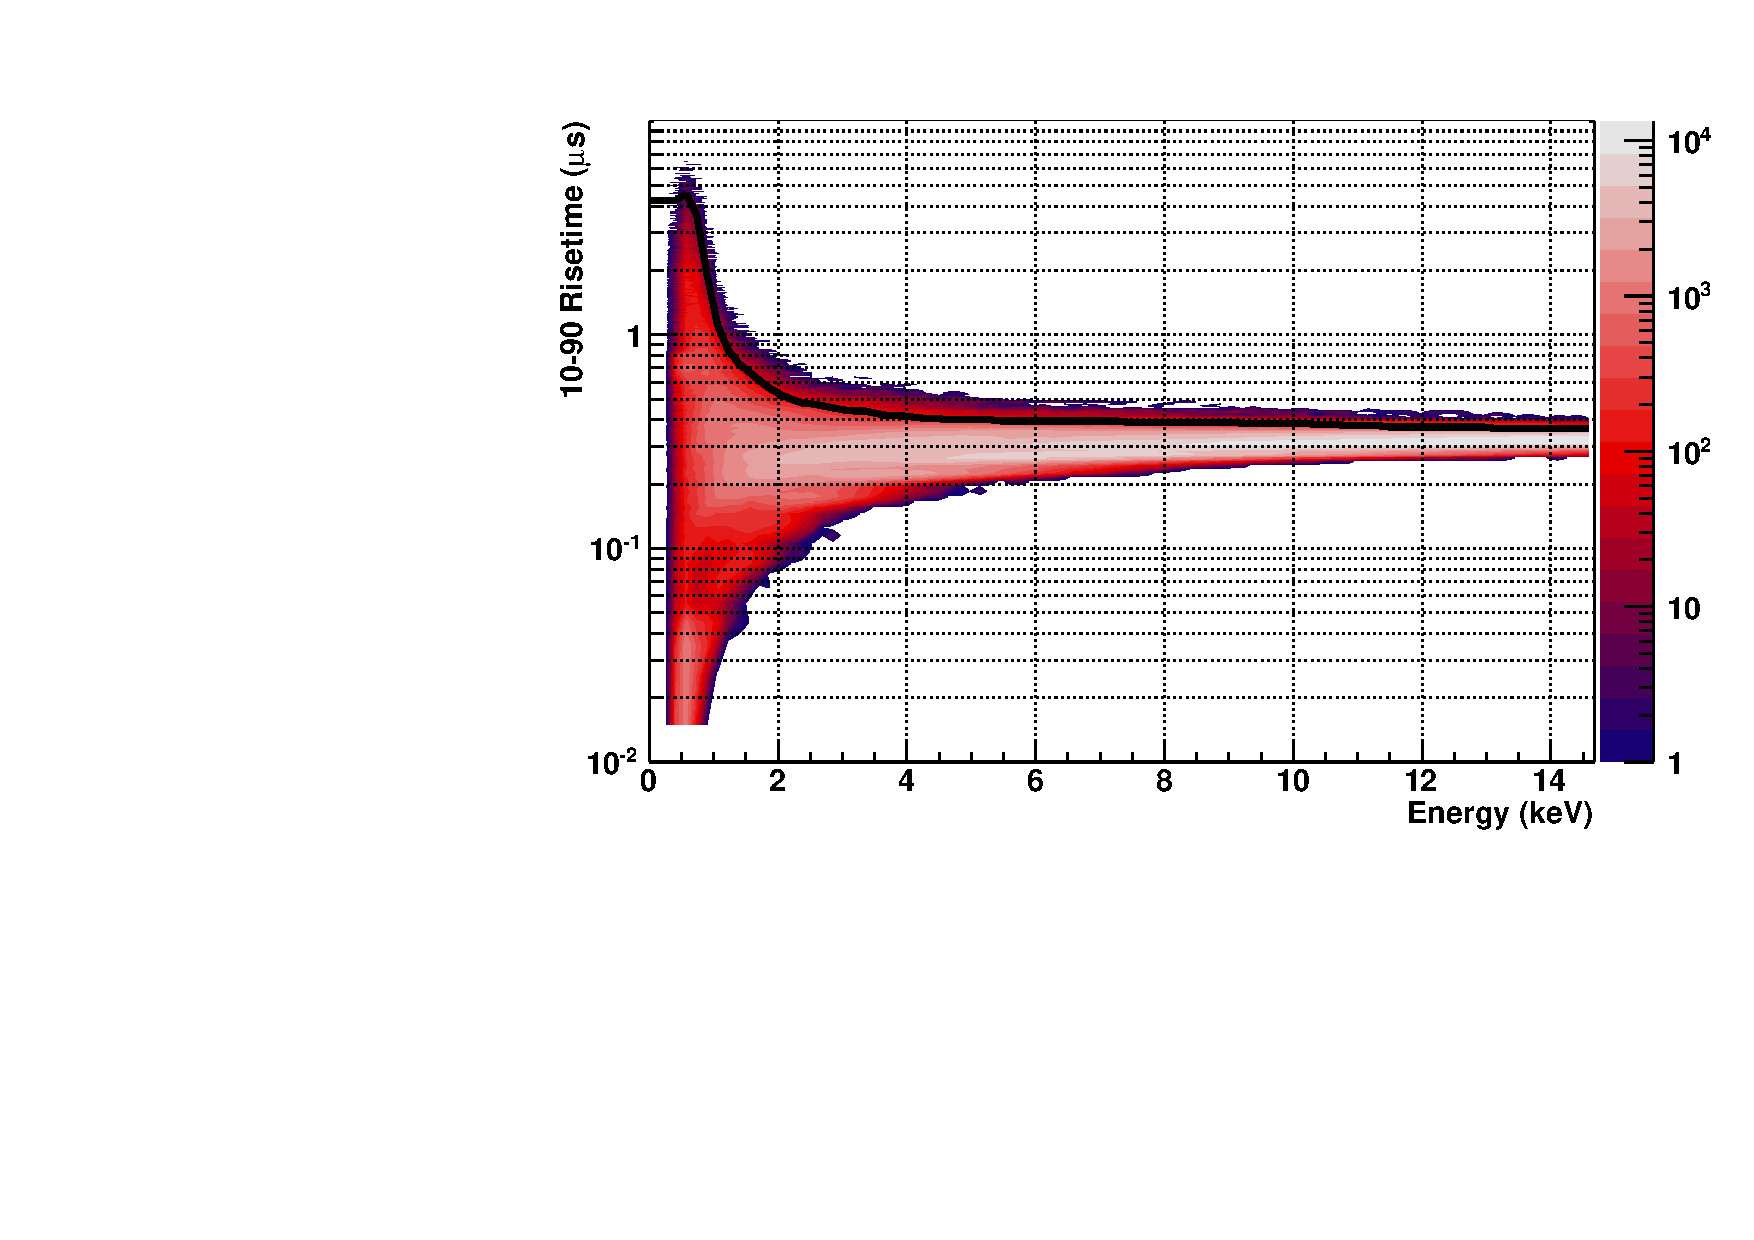
\includegraphics[width=0.9\textwidth]{risetime_cut_chan5_nice}					
						}
						\subfigure[High-gain channel] {
							%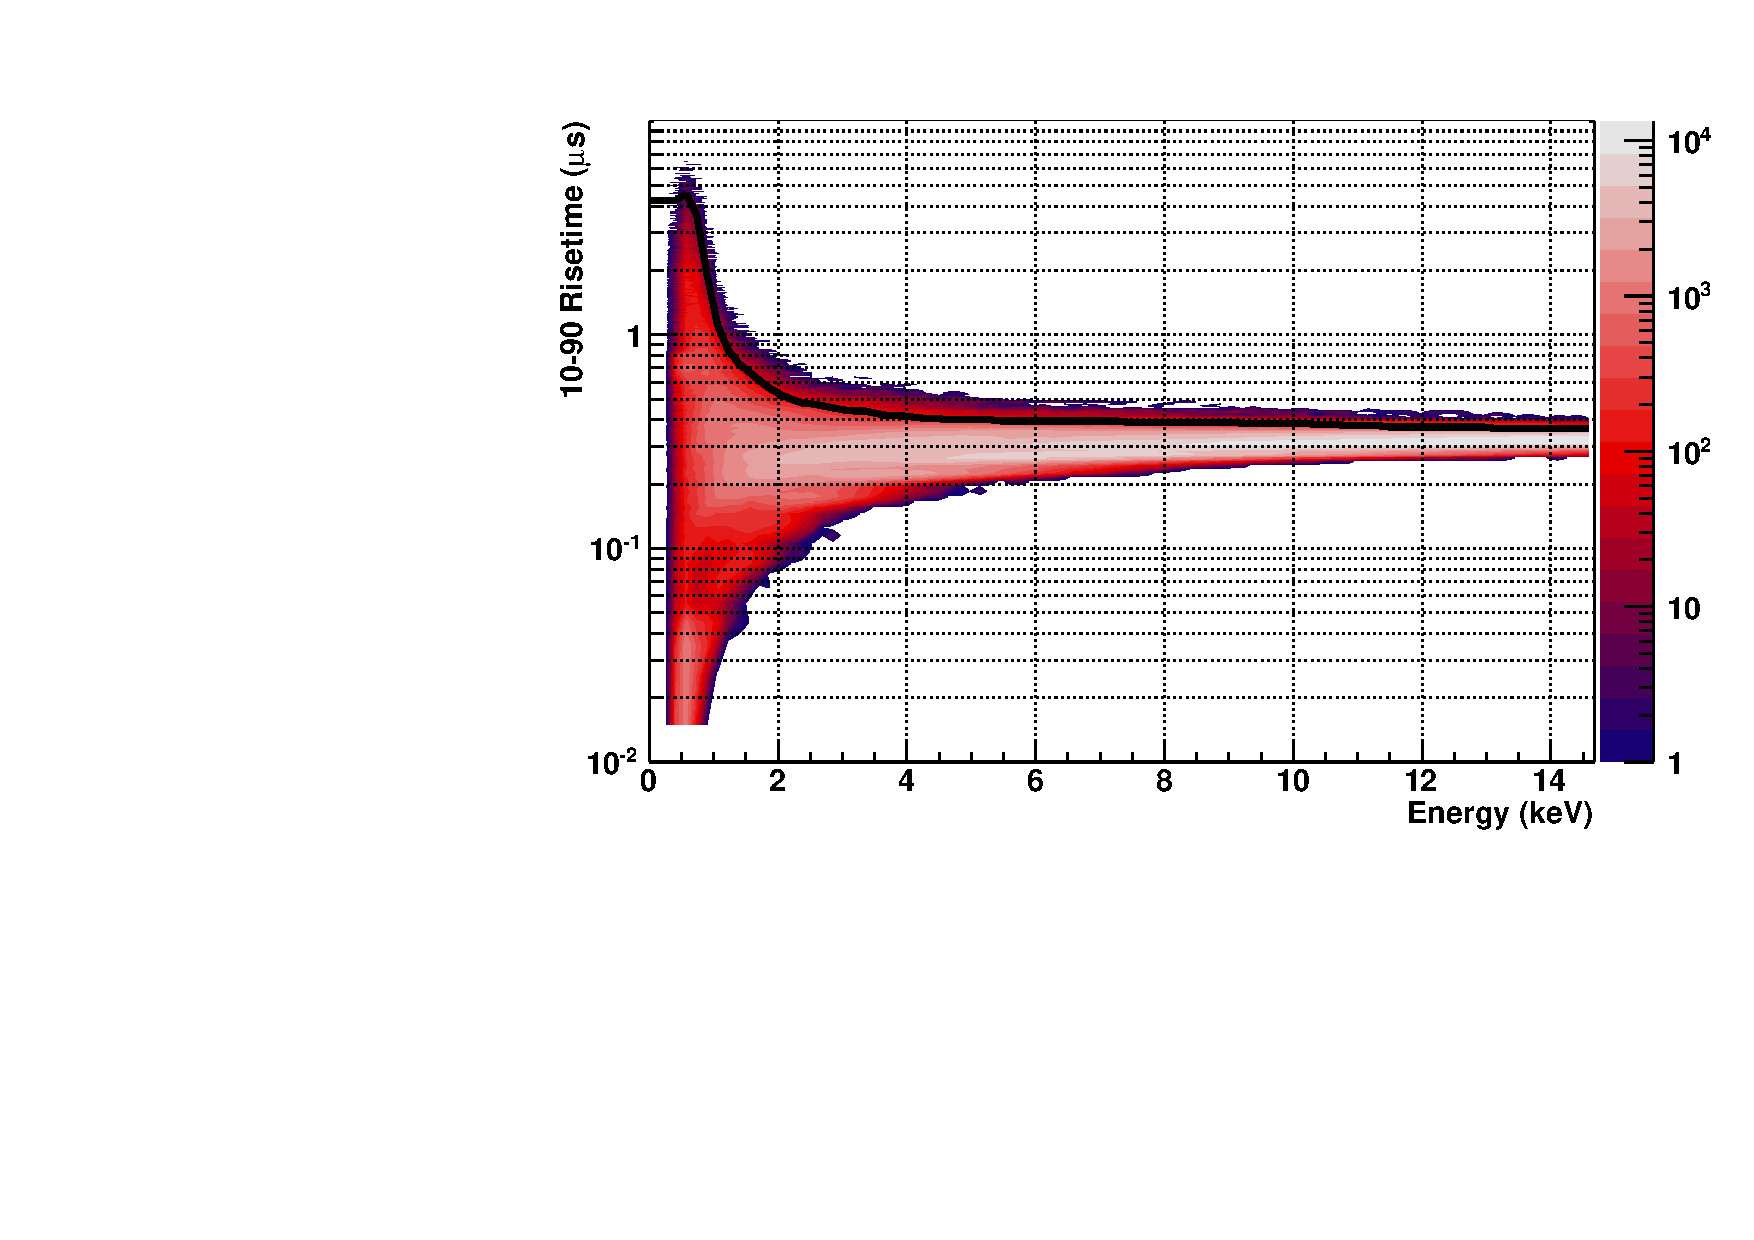
\includegraphics[width=0.9\textwidth]{risetime_cut_chan5_nice}
						}
						
						\caption[Example of fits performed to estimate amount cut by rise-time cuts]
						{Example of fits performed to estimate amount cut by rise-time cuts.}
						\label{fig:BeGeFitExample}
					\end{figure}
	
					\begin{table}
					\centering
						\begin{tabular}{l|r}
							Isotope & Energy \\
							\hline
							\hline
							$^{65}$Zn L-capture & 1.1~keV \\
							\hline
							$^{68,71}$Ge L-capture & 1.299~keV \\
							\hline
							$^{65}$Zn K-capture & 8.979~keV \\
							\hline
							$^{68,71}$Ga K-capture & 9.659~keV \\
							\hline
							$^{68,71}$Ge K-capture & 10.367~keV \\
							\hline
							$^{73,74}$As K-capture & 11.103~keV \\
							\hline
							\hline
						\end{tabular}	
						\caption[Summary of prominent x-ray lines in the BeGe data set]
						{Summary of prominent x-ray lines in the data set.}
						\label{tab:XRayLines}
					\end{table}


					\paragraph{High-energy results}

The results for the low-gain channel are given in Figure~\ref{fig:RTSimLowGainResults}.  The higher-energy x-rays ($>8$~keV) behave well at the higher acceptance percentages ($\ge$90\%), though the agreement becomes worse at lower acceptances as the lines tend to retain a larger percentage of counts than expected.  The lower-energy L-capture lines of \gersixeight~and \znsixfive~follow the general trend, but the wide error bars due to the large covariance of the parameters of these lines makes it difficult to conclude anything more specific.  This large covariance is due to the lack of resolution of the low-gain channel at these low energies, so the high-gain channel is required to test this cut.  The amplitudes of the background components also behave as expected, showing a reduction significantly greater than 99\% for a 99\%-acceptance risetime cut.  The fit exponential constant, $c_{1}$, demonstrates a marked shift when the rise-time cut is initially implemented, but is consistent between the different rise-time cuts (see Figure~\ref{fig:RTLowGainExpConstant}).  This suggests that the calculated acceptance contours are consistent near threshold.  


						\begin{sidewaysfigure}
							\centering
							\subfigure[Exponential Constant, $c_{1}$l]{
								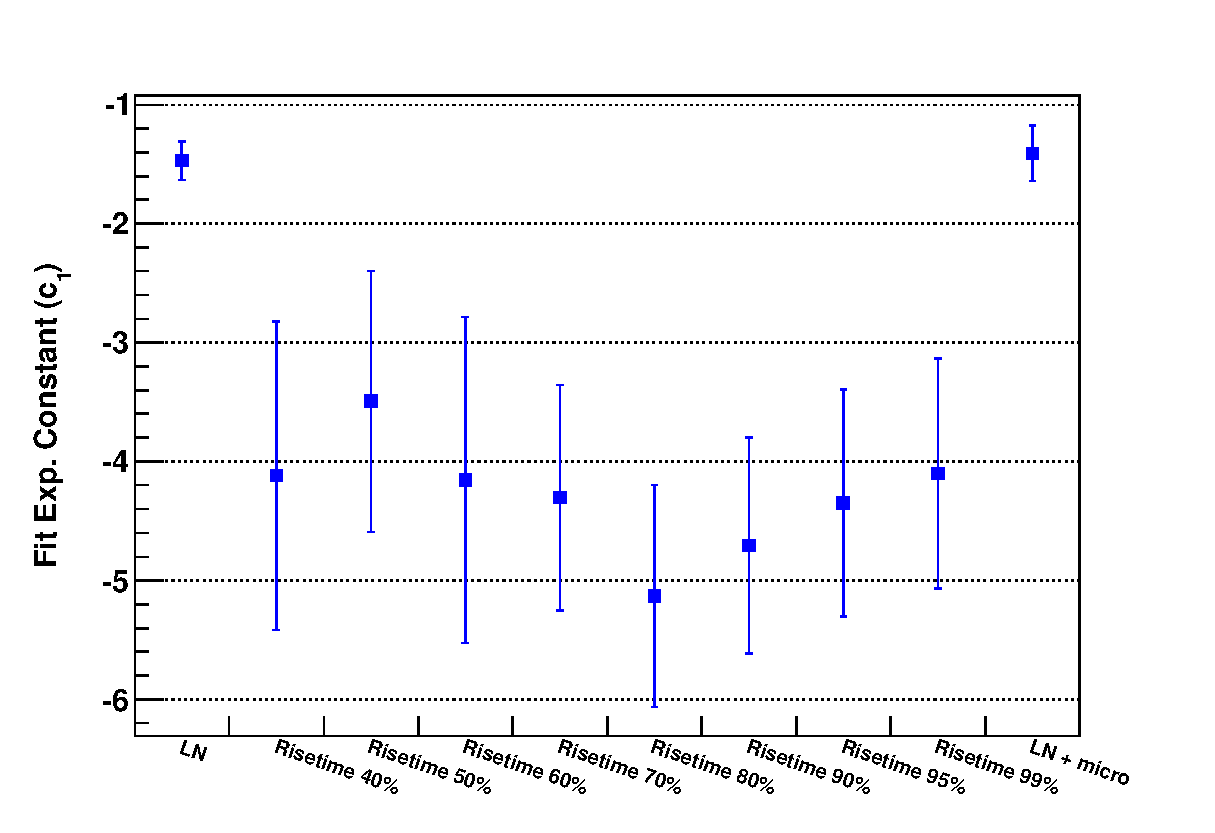
\includegraphics[width=0.46\textheight]{ExpConstant}
								\label{fig:RTLowGainExpConstant}
							}
							\subfigure[X-rays]{
								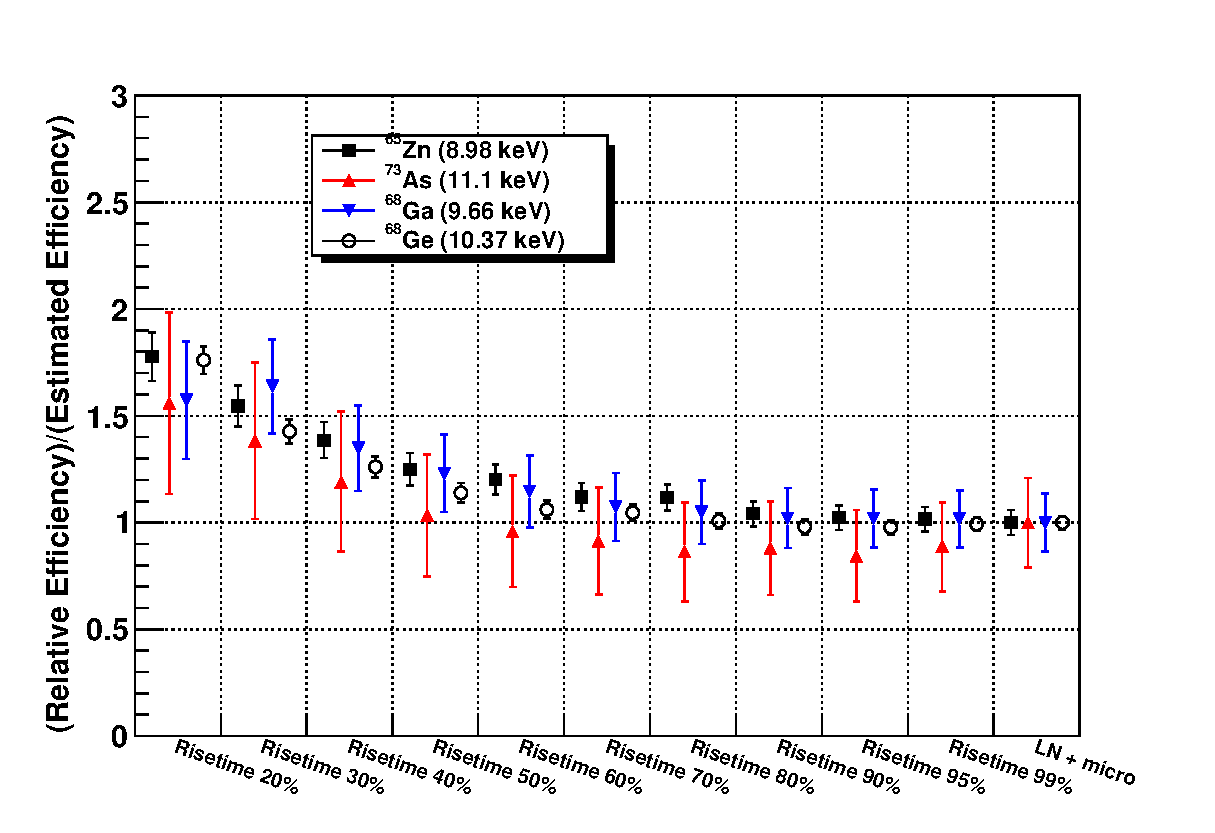
\includegraphics[width=0.46\textheight]{GammaLines}
								\label{fig:RTLowGainXrays}						
							}
							\subfigure[Low x-rays]{
								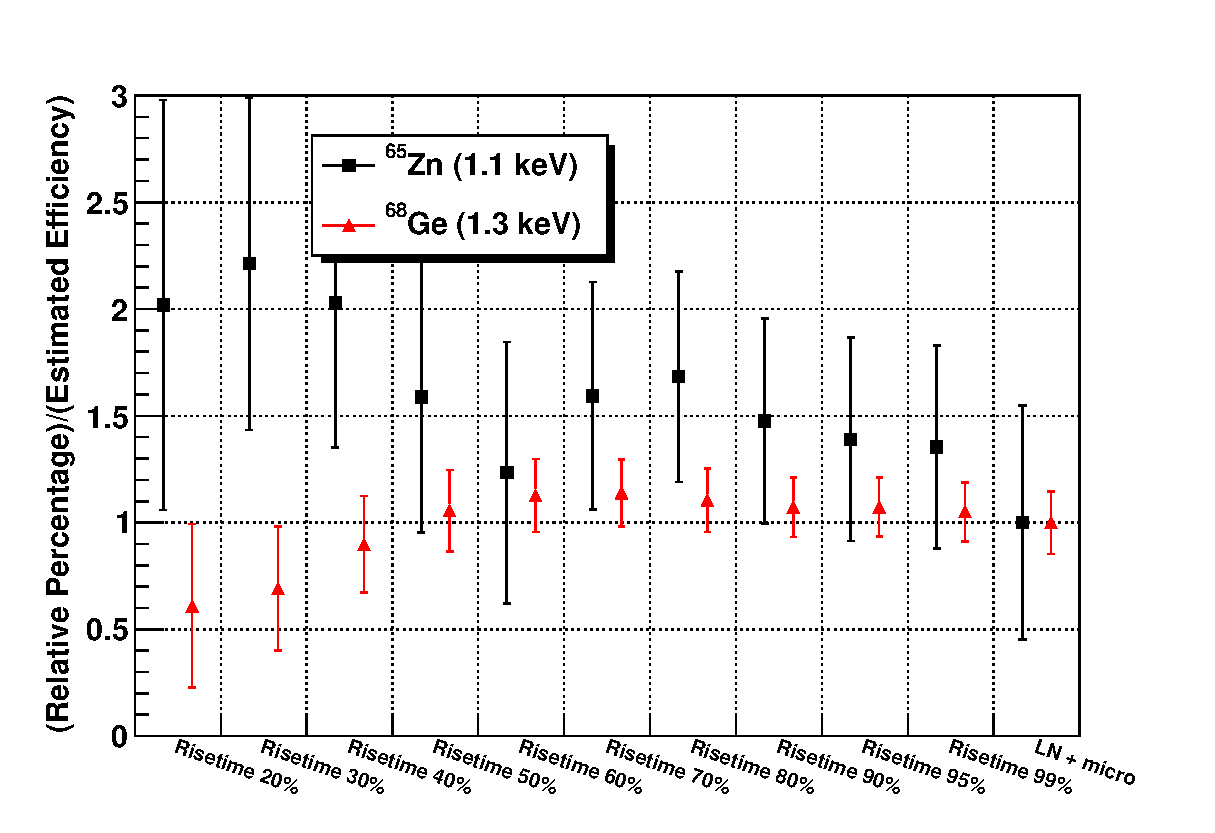
\includegraphics[width=0.46\textheight]{LowHighGammaLines}
								\label{fig:RTLowGainLowXrays}						
							}												
							\subfigure[Background components]{
								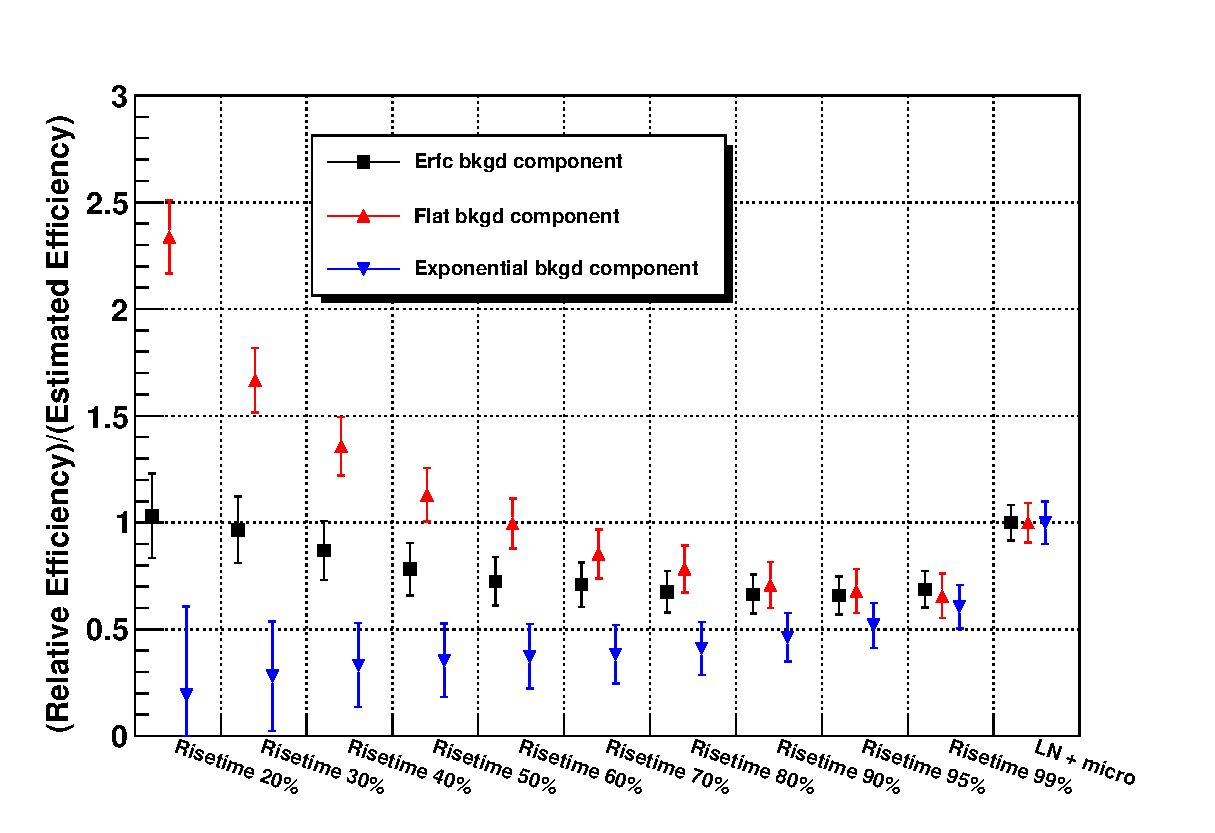
\includegraphics[width=0.46\textheight]{BackgroundComponents}
								\label{fig:RTLowGainBkgd}						
							}														
							\caption[Simulation results for low-gain BeGe channel]
							{Simulation results for low-gain channel.}
							\label{fig:RTSimLowGainResults}
						\end{sidewaysfigure}

					\paragraph{Low-energy results}

Results for the low-energy channel are shown in Figure~\ref{fig:RTSimHighGainResults}. The conclusions for this channel set are similar to the high-energy channel set.  The enhanced resolution of the high-gain channel has reduced the size of the error bars for the L-capture lines and the reduction of the amplitudes of the lines is consistent with the expected acceptances.  The amplitudes of the different background components agree with the amplitudes calculated for the high-energy channel.  The larger error bars on both the background components are because the flat component has fewer constraints: the size of the flat region is significantly smaller in the high-gain channel than in the low-gain channel.  


						\begin{sidewaysfigure}
							\centering
							\subfigure[Exponential Constant, $c_{1}$l]{
								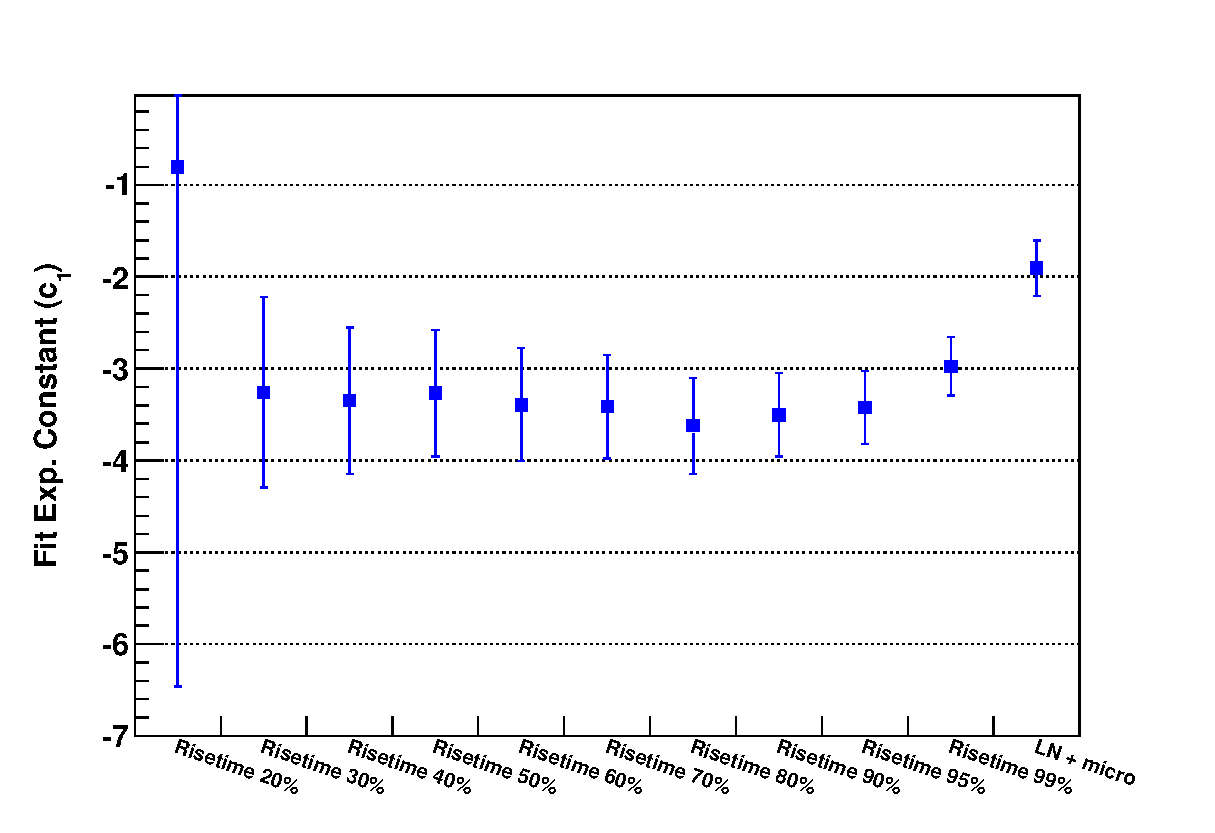
\includegraphics[width=0.46\textheight]{LowExpConstant}
								\label{fig:RTHighGainExpConstant}
							}
							\subfigure[X-rays]{
								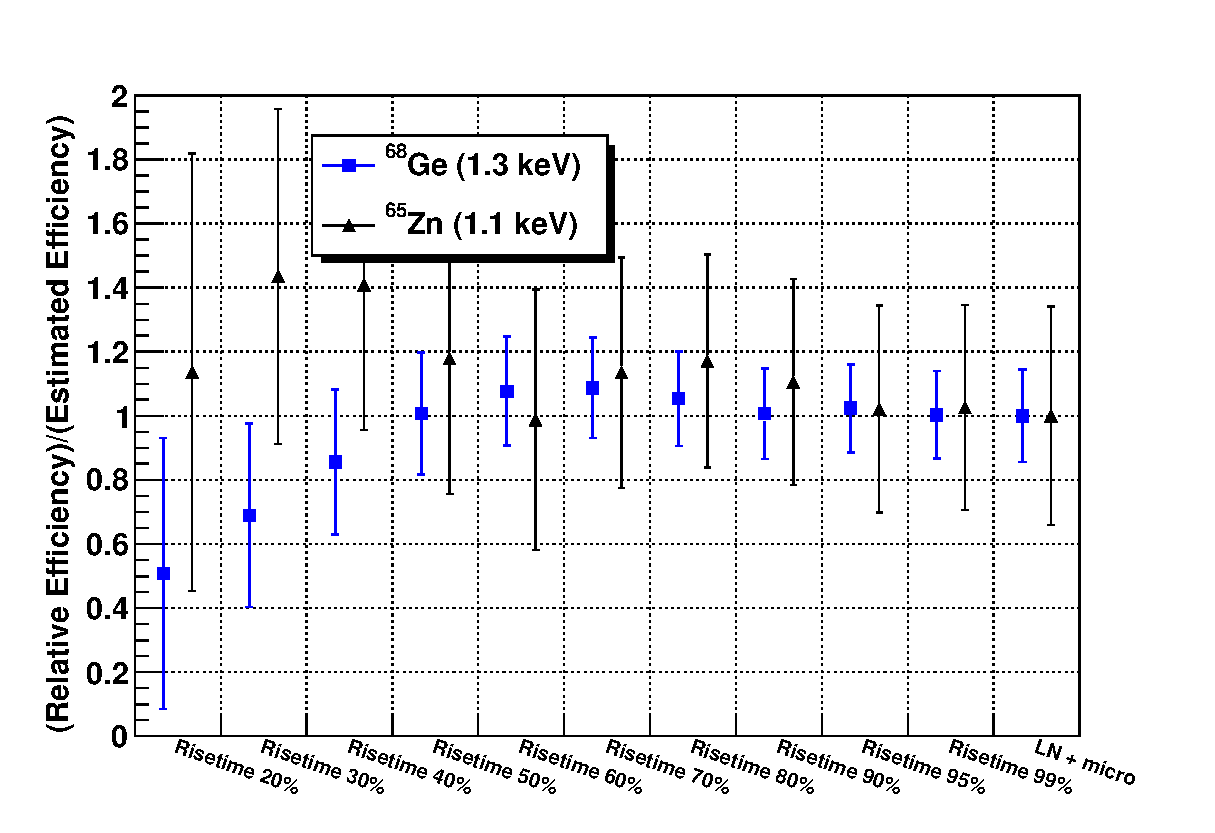
\includegraphics[width=0.46\textheight]{LowGammaLines}
								\label{fig:RTHighGainXrays}						
							}		
							\subfigure[Background components]{
								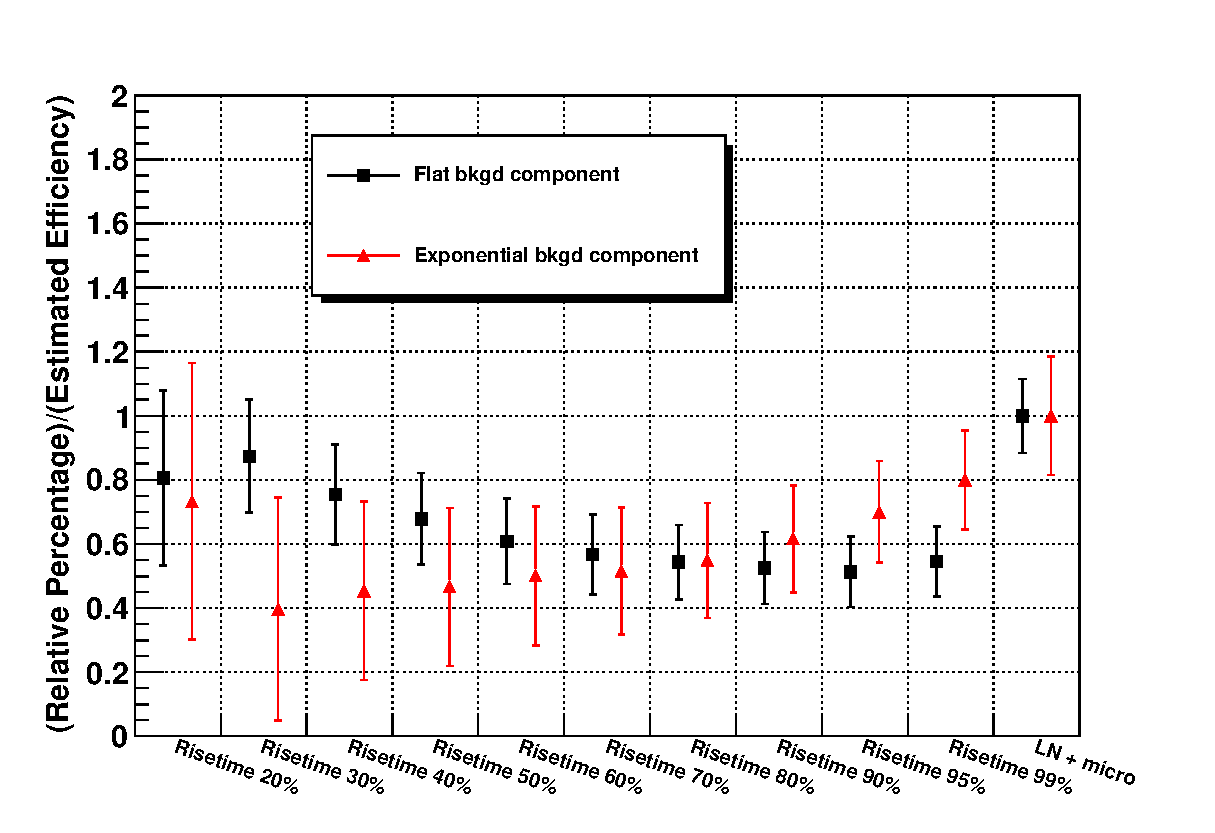
\includegraphics[width=0.46\textheight]{LowBackgroundComponents}
								\label{fig:RTHighGainBkgd}						
							}														
							\caption[Simulation results for high-gain BeGe channel]
							{Simulation results for high-gain channel.}
							\label{fig:RTSimHighGainResults}
						\end{sidewaysfigure}

FixME - Add discussion on Rise-time cuts regarding its interpretation as a fiducial volume cut and the estimate of the mass difference that went along with this.


	\section{Low-energy features}
	\label{sec:BeGeLowEnergyFeatures}
	
	Here, we discuss how the investigation of several parameters in the low-energy region to try and obtain an idea of from where they might arise.

FixME - Flesh out low-energy features, discuss from where these might arise, how one might actually test such hypotheses, and how we got around it for this stage.

	\section{Cuts discussion}
	\label{sec:BeGeCutsDiscussion}

FixME - Add figure showing what is cut out for each cut.

	\section{Conclusions}
     	\label{sec:CutConclusions}		
	

FixME - Discuss the final data sets, the calculation of the total efficiencies, discuss how these may be used (point to the next chapter).  
  
FixME - Discuss possible moves forward in the future, i.e. how to generate a better data set, what sort of data you'd like to take, (measurements), etc.  			
	% At this point, go through and discuss how each of the systematic of each of these cuts must be tested.
	% Discuss how this methodology is later applied to a real dat set.  
	% Discuss other possibilities for reduction in noise, especially with respect to preamp traces.


